\section{Overview}
This section will provide an overview of the chosen solution using rich pictures.

The server-station relation is shown in \figref{fig:ServerRichPicture}. 
The server contains collected information from each station, such as bookings, amount of available bicycles at stations, and usage statistics that allow for improvement.
It provides this information to the users of the system through a webpage.

\begin{figure}[h]
\centering
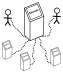
\includegraphics[scale=3]{serverrichpicture/server.pdf}
\caption{Rich picture of the server and the associated stations.}
\label{fig:ServerRichPicture}
\end{figure}

The stations receive the information that allows it to do its function. The stations share with the central server, this can be seen in more detail, such as the amount of available bicycles, this can be seen in \figref{fig:StationRichPicture}.

\begin{figure}[h]
\centering
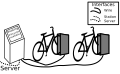
\includegraphics[scale=3]{stationrichpicture/station.pdf}
\caption{Rich picture of the station and the bikes.}
\label{fig:StationRichPicture}
\end{figure}

The bicycles themselves only have one function, with the provided dock (that provides the locking mechanism), in that they can either be locked or unlocked and the station detects this and counts the locked bicycles as being present and unlocked bicycles as not being present. 
This can be seen in \figref{fig:Bicycles}.

\begin{figure}[h]
\centering
\begin{subfigure}[b]{0.3\textwidth}
\centering
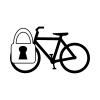
\includegraphics[scale=1]{Bicyclewithlock/bicylewithlock.pdf}
\caption{Locked bicycle.}
\label{fig:BicycleLocked}
\end{subfigure}
~
\begin{subfigure}[b]{0.3\textwidth}
\centering
\includegraphics[scale=1]{Bicyclewithoutlock/bicylewithoutlock.pdf}
\caption{Unlocked bicycle.}
\label{fig:BicycleUnlocked}
\end{subfigure}
\caption{Rich picture of bicycle.}
\label{fig:Bicycles}
\end{figure}